\chapter{Implementation and Evaluation}
\label{chap:eval}
\section{Imlementation of the inference engine}
\begin{figure}
    \centering
    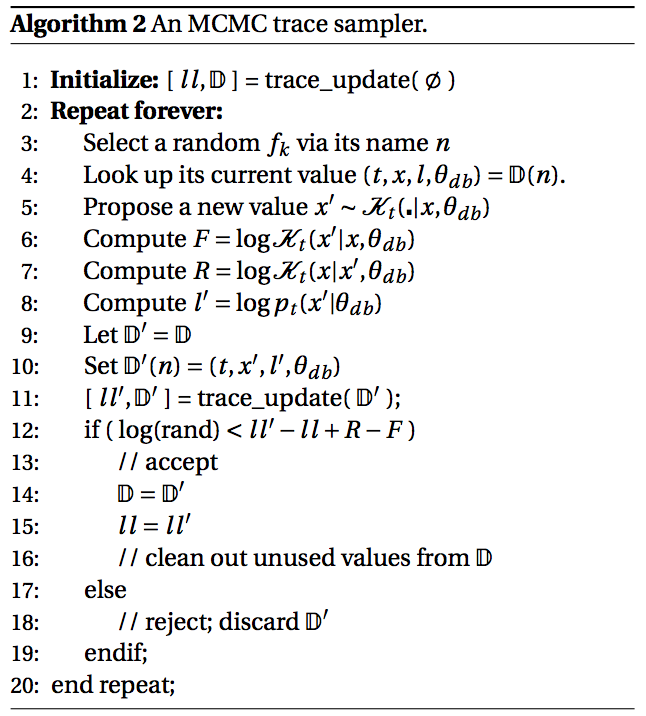
\includegraphics[width=0.7\textwidth]{figures/trace1.png}
    \caption{An MCMC trace sampler.}
    \label{fig:trace1}
\end{figure}

\begin{figure}
    \centering
    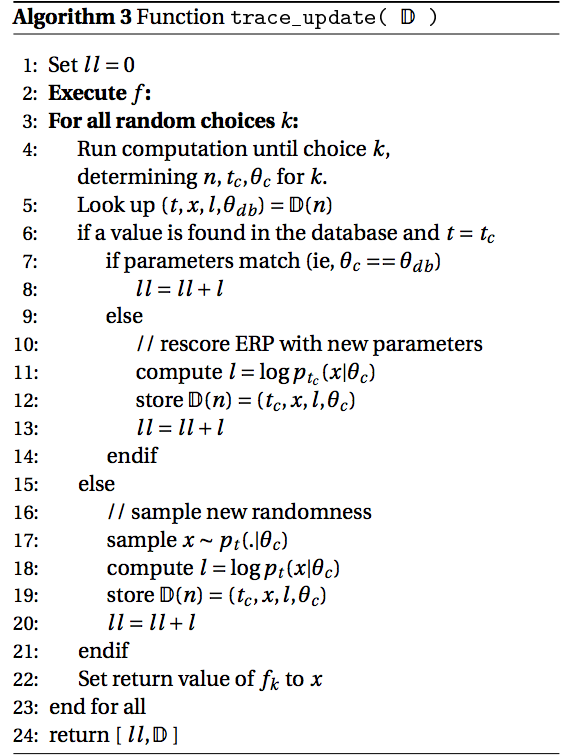
\includegraphics[width=0.7\textwidth]{figures/trace2.png}
    \caption{Algorithm for trace update}
    \label{fig:trace2}
\end{figure}

In the implementation of the MH alorithm in our inference engine, we leverage the approach proposed by ~\cite{lightweight}, which memorized trace information and update trace iteratively as illustrated in Figure ~\ref{fig:trace1} and Figure ~\ref{fig:trace2}. 

There are some other methods to implement an inference engine such as \cite{nonstandard}, which showed how \textit{nonstandard interpretations} of probabilistic programs can be used to perform efficient inference algorithms. In their method, infromation about the structure of the distributions (which is the dependencies or gradients in the probabilistic graphical models) is derived as monad-like side computation as the same time of executing the program. Meanwhile, the interpreations can be coded easily with some special-purpose objects and operator overloading. They promoted the inference efficiency perfomance by using the structure information of distribution as part of the variety of infreence algorithms.

Additionally, because of the program is in a machine-readable form, various of techniques from compiler design and program analysis can be used in the inference engine. ~\cite{gordon2013} designed a new model-learner pattern for Bayesian reasoning. In their work, a new probabilistic programming abstraction was proposed, a typed Bayesian model, based on a pair of probabilistic expressions for the prior and sampling distributions. Also, ~\cite{dataflow} presented a new algorithm for Bayesian inference over probabilistic programs, whihc is based on data flow analysis techniques from the program analysis community.


\section{Experiments}
We have evaluated several examples in the framework. 
\subsection{Flip example}
For the flip example as is showed in ~\ref{fig:flip_eg}, the benchmark is as below:

\subsection{example}